%
% 2018 7. Разработка ядра логического вывода конфигураций каркасов функциональных блоков информационной системы по комплексной модели MDA.
% 2019 7. Разработка технологий и инструментальных средств создания размеченных документов на основе интерпретации комплексной платформонезависимой модели информационной системы.
% 2020 7. Разработка специализированного интерпретатора платформонезависимой модели, ориентированного на поддержку современных средств разработки интернет-приложений, функционирующих в среде Linked Open Data.
\documentclass[conference]{IEEEtran} \IEEEoverridecommandlockouts

% The preceding line is only needed to identify funding in the first footnote. If that is unneeded, please comment it out.
\usepackage{cite} \usepackage{amsmath,amssymb,amsfonts} \usepackage{algorithmic} \usepackage{graphicx} \usepackage{textcomp} \usepackage{xcolor} \def\BibTeX{{\rm B\kern-.05em{\sc i\kern-.025em b}\kern-.08em T\kern-.1667em\lower.7ex\hbox{E}\kern-.125emX}} 

%\usepackage[T1]{fontenc}
%\usepackage[utf8]{inputenc}
\usepackage{luatextra} \usepackage{currvita} \usepackage{minted} 

%\usepackage{ulem}
%\usepackage[]{geometry}
% \usepackage[a4paper,margin=2cm]{geometry}
\usepackage{multicol} \usemintedstyle{bw} \usepackage{enumitem} 

%\usepackage{indentfirst}
\setminted{fontsize=\small} 

\providecommand{\sout}[1]{} 

% *** CITATION PACKAGES ***
%
%\renewcommand\cite[1]{[[#1]]}
\usepackage{hyperref} \hypersetup{ 

% bookmarks=true,         % show bookmarks bar?
unicode=true, pdftoolbar=true, pdfmenubar=true, pdffitwindow=false, pdfstartview={FitH}, 

% non-Latin characters in Acrobat’s bookmarks% show Acrobat’s toolbar?% show Acrobat’s menu?% window fit to page when opened% fits the width of the page to the window%pdftitle={},    % title
%pdfauthor={Author},     % author
%pdfsubject={Subject},   % subject of the document
%pdfcreator={Creator},   % creator of the document
%pdfproducer={Producer}, % producer of the document
%pdfkeywords={keyword1, key2, key3}, % list of keywords
%pdfnewwindow=true,      % links in new PDF window
colorlinks=true, linkcolor=black, citecolor=black, filecolor=black, urlcolor=black, final=true } 

% false: boxed links; true: colored links% color of internal links (change box color with linkbordercolor)% color of links to bibliography% color of file links% color of external links
\setmainfont{Times New Roman} 

\begin{document} \title{Представление трансформаций MDA в виде логических объектов} 

% \titlerunning{Implementation of a QMS with MDA}
\author{ \IEEEauthorblockNЕвгений Черкашин, Алексей Шигаров, Вячеслав Парамонов} \IEEEauthorblockA{\textit{Институт динамики систем и теории управления СО РАН,} \\ \textit{Иркутский научный центр СО РАН} \\ Ул. Лермонтова, д. 134, г. Иркутск, Россия, 664033\{eugeneai,shig,slv\}@icc.ru} } 

% \tocauthor{Evgeny Cherkashin, Alexey Shigarov, Viacheslav Paramonov, Ljubica Kazi}
% \authorrunning{Evgeny Cherkashin, Alexey Shigarov \emph{et al.}}
% \email{\{eugeneai,shig,slv\}@icc.ru, ljubica.kazi@gmail.com}}
\maketitle

\begin{abstract} Рассматривается задача моделирования программного обеспечения, которая представлена набором исходных моделей, а трансформация -- на основе логического вывода. Исходные модели преобразуются в RDF-графы и, затем, обрабатываются системой знаний, структурированной в сеть объектов. При этом существует возможность использования различных нотаций, например таких, как UML, SysML, CMMN, BPMN2.0, графов RDF и результаты анализа исходного кода других систем, если реализовать соответствующий модкль преобразования. Объекты представлены в языка программирования LogTalk. Сценарий трансформации задается в виде объектов, делающих запросы друг к другу, и реализующих, в целом, парадигму модельно--управляемой архитектуры (Model Driven Architecture). 

% 70-150 words
Использования такого подхода к трансформации позволяет разрабатывать исходный код каркасов программных систем еще на этапе общего дизайна, включать в трансформацию различные источники модельных данных, задавать и структурировать знания.  Приводится пример использования разрабатываемых инструментов для представленя модулей прикладного пакета Mothur в виде блоков визуального потокового программирования системы Rapidminer \end{abstract} 

\begin{IEEEkeywords} модельно-управляемаяархитектура, логический вывод, 	RDF, LogTalk \end{IEEEkeywords} 

\section{Введение} \label{sec:intro} 

% The simplest approach to a system improvement consists of the repetitive execution of the following steps over a level of organization under reingeneering:
% \begin{enumerate}
% \item imaging the target state of the system (future),
% \item comparison with the present state,
% \item assessment of the deviations from the target state,
% \item planning set of actions for reaching the target state,
% \item performing the planned set of actions,
% \item control of the achieving the target state by, e.g., checking the set of target criteria.
% \end{enumerate}
% Business process (BP) reingeneering usually starts from a technical audit (TA), the process of a system analysis of an organization structure, its problems and resources \cite{techaudit}.  The result of the TA is set of text documents describing the present state of the organization and its BPs on the various levels (social, administrative, technical, and physical).  The set comprises specifications of organization structure, BP models (AS-IS, TO-BE), target state requirements and restrictions, etc.
% [[Specification structure]]
% [[[Point of views: people resources, marketing, technology, IT, finance]]]
% [[Gathering information]]
% There are three general creative roles of stakeholders involved in the improvement and revealed during TA: \emph{problem owner}, \emph{knowledge owner}, and \emph{problem solver}.  Problem owner is the agent (person), who recognizes the problems in the current state.  This role describes future target state as a ranged list of \emph{requirements} and \emph{restrictions}.  Knowledge owner describes the states in technical terms of the problem domain.  The description contains structure of BPs, their sequences, parameters, causal relationship, control processes, etc.  Problem solver searches and devices a problem solution, relying on a problem solving methodology, respecting interests of the problem owner, and information acquired from knowledge owner.
% [[[How we can represent specifications as IT SUBSYSTEM of an existing system? dring the process of improvement]]]
% [[[Application of the nowadays modeling notations in specifications for the low levels]]]
% .....MOD to be improved with more expressive but complex notions of SysML (System Markup Language), BPMN--2.0 (Business Process Modeling Notation) and CMMN (Case Management Modeling Notation).  SysML used to describe organizational and administrative structures in higher degree of abstraction with respect to UML2, which is used at administrative and technical levels, and in the same time to be more detailed.  The usage of these modeling notation will allow to describe the present organizational structure more formally and precisely as a Computational Independent Model (CIM) and Platform Independent Model (PSM) of MDA paradigm, resulting the bridge between specifications and IT resource under development.
% Heaving described BPs structure and flows of an organization in the formal detailed multilevel form in SysML, we could construct an environment of a permanent IS research and development.  At the first stage, a most simple case is being realized: the description could be converted into check lists controlling conditions of business process starting and ending points. The second stage of implementation is the automation of planning after reaching a checked condition.  The third stage is to organize data processing according to the synthesized plan.  In the long run a refined specification description is being integrated with already used software.  All the stages are accompanied with a lot of useful information to be accumulated, forming the quality measurement, knowledge and analysis basis \cite{aiowa}.
% TOO MANY GOALS AND TOO COMPLEX SOFTWARE - SHOULD BE PRESENTED AS A COMPONENT DIAGRAM WHICH CAPTURES THE IDEA AND SERVES AS A BASIS FOR THE LONG-TERM DEVELOPMENT.THE IDEA WRITTEN THIS WAY IS TOO WIDE AND MISTY.
Основная проблема при разработке сложных информационных систем (ИС), а также друхих систем автоматизации протизводства, -- это сложность, коотрая выражается в сложности испольуемых структур данных, интегрированием с другими системани, необходимости этапа быстрого прототипирования на этапе дизайна системы. Если проводить этап порождения исходного кода на этапах дизайна системы, тогда можно порождать прототипы системы сазу же как сформирована формализованна модели разрабатываемой ИС. Существующие CASE-системы реализуют стандартные подходы к проектированию и поэтому не популярны в разработке WEB-приложений, в небольших организациях и стартапах, где процесс разработки характеризуется с высоким уровнем неопределенности требований и спецификаций. 

Полноценная поддержка быстрого прототипирования требует разработки выразительных средств программирования трансформаций из комплекса разнородных моделей, представляющих различные аспекты ИС, например, UML, SysML, BPMN, которые задаются при помощи соответствующих визуальных инструментов.  Программирование трансформаций необходимо стелать близким к обычному традиционной программированию, позволяющему, в частности, создавать из существующих специализированные версии, а также накапливать опыт в библиотеках объектов и компонент. Внедрение объектно-ориентированного программирования позволило бы создавать трансформации, структурируя базу знаний, позволяя проводить манипуляции с наборами знаний, инкапсулировать знания в трансформационные компоненты. 

% This technique should improve generative approaches is due to absence of transformation implementation techniques ``consuming and adapting previous experience'' expressed in transformational libraries, which are also absent.
Модельно-управляемая архитектура (Model Driven Architecture, MDA) -- это наиболее изученный и развитый трансформационный подход, выходящий за ограничения CASE--систем. MDA представляет процесс порождения кода подсистем ИС как многостадийный процесс преобразования исходной визуальной модели. Код генерируется из так называемой платформо-зависимой модели (Platform Specific Model, PSM), которая представляет реализацию ИС с включением специфики программно-аппаратной платформы... PSM получается из платформо-независимой модели (Platform Independent Model, PIM), которая описывает ИС на более абстрактном уровне. Часть PIM порождается из вычислительно-независимой модели (Computational Independent Model, CIM), описывающей ИС и ее окружение на концептуальном, организационном, системном уровнях, абстрагированных, в целом, от преобразования информации и вычислений. 

%Input models are stored in various format, including proprietary ones; they could be converted to OMG standard XMI representation.  XMI is a set of identified structural components,
CIM и PIM обычно задаются набором SysML, CMMN, UML и других визуальных моделей, которые сохраняются стандартным способом в виде XMI-файлов\footnote{XML Metadata Interchange}. Кроме этих моделей дополнительные данные для трансформации могут быть получены из Семантического Веба (СВ), например, определения онтологии, названия сущностей в различных естественных языках, текущее состояние процессов, и так далее. Популярные способы трансформации модели, как ATL\footnote{ATLAS Transformation Language}, основаны на трансформации одной XMI-моделm в другую XMI, а затем уже в код. Привлечение данных СВ достаточно проблематично. 

Мы предлагаем более общий подход, где для всех исходных типов моделей разрабатываются конвертера в формат RDF\footnote{Resource Description Framework}, в стандартное представление данных и знаний в СВ, а трансформация программируется в виде объектно-ориентированной логической программы на языке LogTalk. Это позволяет нам представлять трансформации как сценарии из объектов, обменивающихся сообщениям и запрашивающих модельные данные из графа СВ. Объектное программирование позволяет нам структурировать, управлять базой знаний при помощи инкапсуляции, наследования, расширения и композиции. 

\emph{Объектом} исследования является разработка технологии реализации трансформации как системы знаний такой, чтобы была возможность обработки модельных данных CIM и PIM из разнородных источников. \emph{Предметом} статьи является описание предложенного выше представления данных и методов преобразования моделей. 

\section{Архитектура инструментов MDA} 

% (here we speak about how to convert BPMN, SysML and CMMN models into carcass of an Inform. System... various stages of processing, including input....)
Архитектура средства трансформации основывается на обеспечения единообразия языка правил трансформации язык и [[предикативного]] представления входных данных. Поэтому мы требуем, чтобы либо хранить все входные модели данных в виде графов СВ при помощи соответствующих онтологий, или создавать конвертер, представляющий исходные модели в виде таких графов. Графы хранятся в виде RDF-файлов или загружаются с сервера через точки доступа SPARQL. Общая архитектура средств разработки представлена на рисунке \ref{fig:archi}. 

\begin{figure}[htb] \centering

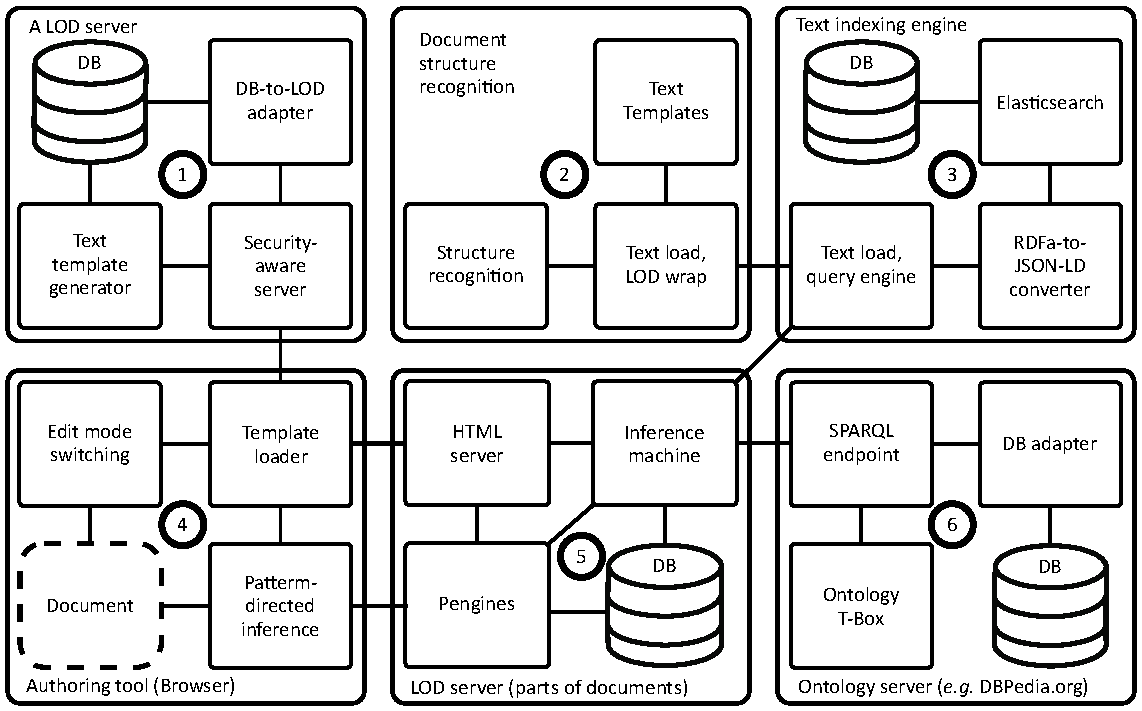
\includegraphics[width=1\linewidth]{pics/architecture-mda-lod-ext.pdf} \caption{Архитектура инструментальных средств трансформации} \label{fig:archi} \end{figure} 

Инструменты MDA состоят из следующих основных компонентов: \begin{itemize} \item сервер исходных моделей (2), который хранит модель данных в виде RDF-троек; \item механизм трансформации (1), который запрашивает данные с сервера моделей и других SPARQL-совместимых серверов (4); \item конвертеры форматов представления моделей CIM (3) и PIM (6); \item сервис полнотекстового индекса (5). \end{itemize} 

Все компоненты взаимодействуют при помощи сетевых протоколов и используют форматы HTML, TXT, XML, JSON в кодировке UTF-8. [[Inference engines also support SPARQL protocol for issuing subqueries]]. 

Подсистема MDA представляет собой набор модулей трансформации (Т--модули). Каждый Т--Модуль в общем случае является параметризованным объектом LogTalk. Объект запрашивает у сервера моделей предметной области.  Сервер построен на базе системы ClioPatria \cite{Clio}.  Объект может запрашивать также другие объекты и другие сервера онтологий. В полученные данные о структуре моделей анализируются и распознаются заданные структурные комбинации.  Результаты кэшируются в состояниях объектов или индексирутся механизмом индексирования текстов. Совокупность состояний объектов представляет собой PSM, которая на последнем этапе трансформации преобразуется в исходный код и начальные данные. 

Исходные данные моделей CIM и PIM преобразуются в графы RDF специальными адаптерами. Например, на рисунке~\ref{fig:archi} CIM (3) сконструирована в редакторе Modelio \cite{modelio} и,  затем, преобразована в тройки в модуле ``Конвернтер XMI в RDF''. Аналогичный конвертер разработан и для PIM, представляемой диаграммами UML. Такой подход позволяет расширять инструмент новыми видами моделями благодаря такой модульности. 

%IF WE EMPHASIZE SYSML, HOW IS IT RELATED TO SEMANTIC WEB TRIPLETS? THIS SHOULD BE EXPLAINED.
Одним из вспомогательных RDF--совместимым источником данных является сервер \texttt{DBPedia.org}, содержащий именованные константы в различных языках, а также полезные отношения сущностей, представленных в Википедии. Эта информация может быть использована для описания свойств элементов пользовательского интерфейса для редактирования объектов ИС, заданных в исходной модели. Например, мы можем использовать данные DBPedia для формирования атрибутов \texttt{title} и \texttt{placeholder} элемента input, а также соответствующий текст метки (label) с учетом локальных настроек пользователя и help-текста. 

% Some UML-structures (OCL) and relations may be interpreted constructively as methods of objects: events, handlers, subscribers, database triggers and selectors (lookups widgets).
\section{Представление данных моделей в RDF} \label{sec:rdf-repr} 

Последние 20 лет разработки технологий СВ привели к созданию стандартов описания большого количества предметных областей, причем большинство из них стандартизованы консорциумом W3C. Наличие этих стандартов позволяет разработчикам ИС использовать глобальные ссылки URI для идентификации конкретных объектов, а также стандарты представления онтологий RDF, RDFa, TTL.  Для большинства сред программирования реализованы библиотеки поддержки технологий СВ. В результате, отрасль ИТ постепенно на глобальном уровне накапливает и стандартизирует знания и данные предметных областей. Именно поэтому, было решено использовать СВ как основной формат представления моделей, что обогащают имеющиеся знания предметных областях дополнительной спецификой. С другой стороны, преобразование сложных древовидных структур, используемых для представления модели, в набор троек, т.е. фактов для машинного вывода, позволяет использовать Prolog в качестве основного механизма трансформации. 

Согласно рекомендациям СВ, каждое описание модели должно быть помечено глобальным URI и, для удобства использования, некоторым синонимом-префиксом. Все отношения и атрибуты должны быть формально описаны в соответствующей онтологии, предпочтительно являющейся стандартной и общедоступной. Имена сущностей и их взаимосвязей, представленных в исходном формате визуального редактора, должны быть конвертируемыми в RDF по запросу во время трансформации. 

\subsection{Определение сущностей} \label{sec:ent-def} 

Идентификация сущностей и их поименование в RDF [[многоаспектно]]. Сущность и отношения существуют, если они где-то определены или где-то есть на них URI-ссылка. Поименование сущностей осуществляется при помощи отношений, \emph{например}, \texttt{dc:title} и \texttt{rdfs:label}. Субъектом отношения является URI сущности, а объектом -- \texttt{литерал} (строка) и метка естественного языка, задаваемая дополнительным атрибутом. Каждый элемент и отношение в нотации модели (метамодели) должны иметь соответствующие обозначения в онтологическом представлении. 

Так как сущности глобально идентифицированы, их наличие в различных моделях обозначают один и тот же объект, например, в BPMN-диаграмме объект -- запись базы данных (или документ) может быть создан из типа, определенного в UML диаграмме классов. Межмодельные ссылки также делаются при помощи URI или префиксной формы RDF \texttt{<prefix>:<identifier>}, где \texttt{<prefix>} -- это аббревиатура подграфа, представляющего модель, в которой задан \texttt{<identifier>}. Большинство средств визуального редактирования UML не ограничивают имена идентификаторов, так же как и семантику структур, предполагая, что она определяется трансформацией. 

%[[ What else it is necessary to describe here?]]
\subsection{Средства расширения семантики моделей} \label{sec:mod-ext} 

Гибкие инструменты моделирования также позволяют дизайнеру расширить семантику структур модели (метамодели). Например, все диаграммы UML поддерживают \emph{стереотипы} (stereotypes), \emph{теговые значения} (tag values) и \emph{ограничения над объектами} (object constrains). Стереотипы задают расширенный набор атрибутов для объекта или связи, например, в диаграмме классов UML стереотипы используются для задания разновидности класса. Если классу назначен стандартный стереотип \texttt{<<interface>>}, тогда класс превращается в определение интерфейса. По умолчанию классам назначен стереотип \texttt{<<class>>}. Те же идею используются, чтобы описать связи между вариантами использования в UML-диаграмме вариантов использования. Один вариант использования может "включать" (\texttt{<<include>>}) или "уточнять" (\texttt{<<extend>>}) другой. Новые стереотипы могут задавать разработчики, например, при разработке ИС удобно использовать ORM\footnote{Объектно-реляционное отображение}, при этом тот факт, что конкретный класс будет отображаться в запись реляционной базы данных можно при помощи назначенного ему стереотипа \texttt{<<RDBMSRecord>>}. В данном случае, класс добавляется в перечень классов, определяющих структуру базы данных, все отношения между такими классами трактуются как реляционные (один-к-одному, один-к-многим, многие-к-многим, обязательные и нет) отношения. Каждой структуре можно назначить множество стереотипов. 

Теговые значения позволяют связать некоторое строковое значение с ключом (строкой), которые так или иначе интерпретируются с процедурой трансформации. Например, самый простой способ назначения полю класса \texttt{age} имени метки в интерфейсе пользователя -- это в диаграмме классов назначить этому полю теговое значение \texttt{interface-label-name} равное строке ``\texttt{Возраст}''. При использовании RDF имена тегов можно задавать в форме \texttt{dc:title}, а значение тега интерпретировать и как литерал и как URI, например, на объект \texttt{DBPedia}. 

Опыт использования стереотипов и теговых значений показал, что назначение определенного стереотипа, как правило, предполагает определение набора одного и того же перечня теговых значений. Стандарт UML версии 2.4 этот момент учтен, и современные средства визуального моделирования позволяют формально определять данный перечень для собственных стереотипов. [[Разработаны специальные интерфейсы пользователя для управления перечнем стереотипов.]] В нашем примере назначение стереотипа \texttt{<<RDBMSRecord>>} классу не позволяет явно задавать соответствующую таблицу, для этого можно использовать теговое значение \texttt{rdbms:table-name}. Таким образом, явная спецификация стереотипов в UML-2.4 -- это мощный инструмент расширения семантики элементов визуальных моделей. 

% [[[Resume of some kind]]]
\subsection{Другие источники модельных данных} \label{sec:other-models} 

При реализации сложных программных систем, их иногда составляют из действующих модулей, спецификации этих модулей могут выступать дополнительными источниками модельных данных. Например, в нашем проекте \cite{bit2019}, основная модель PIM извлекается из исходного кода библиотеки Mothur и преобразуются в ТТЛ-формат. Этот подход требует один раз запрограммировать такой конвертер, и при выпуске новой версии библиотеки мы автоматом получаем новую версию PIM. 

%Formal rules of the source code analysis ad interpretation as PSM can also assist in finding errors in the source code.
% [[PSM libraries....???]]
\section{Исследования--аналоги} 

The most widely used technology of model transformation is ATL (ATLAS Transformation Language) \cite{atl} and its predecessor QVT, an OMG standard \cite{QVT}. The language and its engine supports conversion from one XMI model to another one in the same XMI format. The language structures describe recognition of properties of compositions of the source model and direct construction of new structures in the target model. 

Similar to ATL, Transformation Model Representation Language (TMRL) is developed in \cite{nikita} but oriented on visual representation of a knowledge base with following conversion in various production rules in CLIPS and OWL. The visual presentation of transforming rules are used also in \cite{GT}. In \cite{azis}, ATL is used to transform Computational Independent Model (CIM) represented as BPMN diagram into set of UML diagrams, defining PIM. Paper \cite{Rhazali} proposes a model transformation CIM to PIM for web-applications, where CIM is represented with State and Use case UML-Diagrams logically connected with ATL rules. In \cite{Hamid} is proposed an evaluation of security aspects of distributed applications using MDA description; the evaluation is implemented a logical inference over the MDA synthesized logical security models. The paper \cite{Zdun} is considered a highly decoupled distributed event-driven application environment, whose design and functioning is dynamically controlled by its three-level DSL\footnote{Domain Specific Language} description and MDA transformations, which support change propagation. 

%Paper \cite{Malki} presents a practical approach with four-level ATL-description from HTML-page to a LOD structure (via stage of an MDA PIM). In \cite{uml2owl}, a converter of UML package structures represented in XMI was developed as a XSLT transformation. A wide overview of Western approaches to program transformation is given in \cite{Dama}, a transformation language PROMOL is suggested as well as its logical semantics. OMG proposed ODM standard \cite{odmprof} for knowledge modeling.  A Visual Ontology Modeler \cite{odnext} is being developed for building and verifying OWL ontologies for ODM~1.0, as well as in the reverse direction, ontologies are represented as UML Class Diagrams \cite{odmvis}.
% An XML based specifications are used in representing metadata about web services, WSDL \cite{wsdl}, and the WS-BPEL language \cite{wsbpel} for describing orchestration of web services within execution of an instance of a business process.  The idea of the language is to describe complex systems down to Web Services units, their internal and external structure and behavior, as well as services interaction in the script instance.
Thus, the majority of the presented techniques are closed with respect of XMI file format: the source data and the result of the transaction are represented in it, and it goes beyond only on the stage of the source code generation. Our approach allows one to use other sources (not being presented in XMI) of model information, as well as general purpose libraries in implementation of the transformation engine. Usage of object-oriented logical language LogTalk allows us powerfully structuring and manipulate knowledge base. 

% by means of the object encapsulation, inheritance, and composition.
% \subsection{Ontology Usage in Model Representation}
% \label{sec:use-onto}
% SysML is the dedicated system-level UML-based notation proposed by the OMG. In research \cite{raslan} system design productivity is addressed as one of the main challenges. Some suggested approaches are increasing the level of abstraction and automation, as well as producing executable specifications. In \cite{natale}, model driven development is used for the construction of complex embedded systems integrating software and firmware. A SysML system model is devised according to the platform-based design paradigm, in which a functional model of the system is paired to a model of the execution platform. Subsystems are refined as Simulink models or hand-coded in C++.
% The SysML standard is attracting more attention of hardware designers as UML and SysML have been used to automatically generate an HDL code written in SystemC, Verilog and VHDL. In \cite{boute}, contrarily to the existing works, authors propose the new reverse engineering approach to generate SysML definition of block and internal block diagrams from VHDL code. Code generation is done on the basis of a set of well-defined mapping rules between SysML and VHDL concepts.
% UML profiles like SysML and MARTE have been a major research topic in electronic system design, but are mainly applied for specification and analysis in early design phases.  Research \cite{mish} addresses the problem of the High-Level Synthesis (HLS), \emph{i.e.} physical implementation aspect of electronic systems, which need diversity of design models and levels of abstraction.  To overcome the conflict between a higher degree of abstraction and necessary details for further synthesis, modular interfaces are introduced as object-oriented synthesizable technique. In \cite{mish}, SysML is used as an adequate modeling language for modular interfaces and C/C++/SystemC-based HLS. Authors extended SysML with annotations for synthesizable SystemC and high-level synthesis constraints and implemented a code generation scheme to achieve design flow automation. They used SysML editor Artisan Studio with industrial case study to demonstrate the applicability of SysML as a front-end for HLS.
% In \cite{tom16} UML/SysML is used to model avionics.  The implementation language is C\# with using libXML for XMI import and processing.  Generated objects represent each syntactic element (\texttt{struct}, \texttt{enum}, function, \emph{etc.}), which represents the target source code.  Authors implemented only State Machine diagram transformation.
% % \cite{fab} % the lost reference
% Some experience of representing document flows are obtained by commercial software vendors developing Directum, Documentum systems automatizing Russian municipal institutions and state corporations.  Directum uses SysML state--like block diagrams to define flow of documents and the ISBL object-oriented language to express sophisticated behavior.
% % NOT ONLY THIS, THERE IS MORE NEEDED IN THE RELATED WORK SECTION: BUSINESS PROCESS MANAGEMENT SYSTEMS, BUSINESS RULES MANAGEMENT SYSTEMS, WORKFLOW MANAGEMENT SYSTEMS.
% In our research we focus on representation of ISO 9001 entities in SysML and other DSLs translatable to RDF, and the MDA transformation logical inference representable as LogTalk objects.
% \section{SysML representation of QMS}
% QMS is represented in SysML with nine diagrams \cite{sysmlpres}.  QMS requirements is represented with new (with respect to UML) \emph{Requirement Diagram}, describing stated structural and logical constraints. Structural aspects are represented with following UML2 diagrams:
% \begin{itemize}
% \item \emph{Block Definition Diagram} decomposes structure of activities, attributes and objects on elements;
% \item \emph{Internal Block Diagram} models interaction of the decomposed elements and their data flow; its descendant new \emph{Parametric Diagram} describes model of block attribute relationships;
% \item \emph{Package Diagram} organizes models in packages in various ways.
% \end{itemize}
% Behavioral aspect of a QMS is expressed with UML2
% \begin{itemize}
% \item \emph{Use Case Diagram}, which expresses functions of the system and their mutual relationships;
% \item \emph{State Machine Diagram} defines the states of the blocks and transitions between the states;
% \item \emph{Sequence Diagram} describes the order of messages between blocks and actors;
% \item \emph{Activity Diagram} represents computational process of converting data enclosed in blocks.
% \end{itemize}
% BPMN2.0 diagram is used to describe imperative procedures, it is very expressive diagram representing functions and involving agents, together with their relationships.  CMMN represents declarative aspects of the QMS especially data structures, processing stages, events and check points (milestones).  Adding BPMN2.0 and CMMN diagrams to SysML diagram set creates a redundancy, but in the same time it allows one to use more rich tool set for QMS modeling.
\section{Technique of Transformation Implementation} \label{sec:tech-imp} 

The main idea behind implementation of transformation engine is an usage of an object logical programming language meeting the following constraints: \begin{itemize} \item support multiple sources of model data, \item first-order language for definition of the transformation, \item transformation is represented as rules, \item rules should be encapsulated in objects, \item objects should query other objects for results, \item means for transformation configuration and scenario description, \item knowledge manipulation, including composition, \item expression and query of RDF entities. \end{itemize} 

%The multiplicity of source data is archived with conversion of source structures to RDF triple sets, and object orientation of transformation representation: objects are encapsulations of model data.
SWI-Prolog with macro package LogTalk meet these constraints. The LogTalk objects encapsulate Prolog first-order language rules as methods. Each object is respected as a knowledge base of encapsulated rules. Objects can be inherited (as prototypes or classes), parameterized, and composed with \emph{categories}. In inheritance, methods can be reprogrammed implementing refined knowledge set. Configurations are implemented as a prototyping hierarchies: in inheritance, a configuration are refined by replacing and adding new values. Scenarios are implemented as an ordered sets of methods. Finally, SWI-Prolog has a good LogTalk compatible RDF library strongly tied to the language itself. The library represents RDF entities in a W3C compliant way. 

% [[Rule representation in Prolog]]
% Existing popular approaches of implementing Platform independent model (PIM) to Platform specific model (PSM) transformation, taking into account the runtime and other implementation platform features.  The first approach is model-to-model transformation with a model transformation language, such as QVT-X, ATL, \emph{etc.}  In this case PIM and resulting PSM are represented as X MI files.  Model transformation language rules recognizes structures in PIM and construct structures of PSM, having account various \texttt{boolean} conditions calculated with helper rules. The second variant of transformation is realized with Domain Specific Language (DSL) infrastructure \cite{stratego}.  The transformation procedure is presented as translation of one DSL instance, \emph{i.e.} PIM, to an instance in another language.
%Resume
%Our approach is based on common known in AI tools, but requires additional programming of libraries of model transaction objects.
% \subsection{LogTalk as transformation engine}
% \label{sec:logtalk-engine}
% The direct way of a transformation implementation is to use \textsc{Prolog} or a functional language, and we use \textsc{Logtalk}, a macro package of Prolog.  The main advantage of the language usage is knowledge structuring thanks to its object-orientation.  Objects are used for representation of the source PIM model and the resulting PIM structures as well as source code generators.  Moreover, the transformation rules are easily integrated with libraries processing LOD and LOD warehouses.
\subsection{SWI-Prolog Semantic Web Library} \label{sec:swi-sw} 

SWI Prolog standard distribution contains library for RDF processing. The library represents URI as a corresponding functor with atom argument. This structure can be constructed with a special form \texttt{<namespace>:<identifier>}. Library contains predicates for loading graphs from files and internet sites, store them in various text based and binary formats for later use. 

The library support queries for the graphs as a predicate query and as SPARQL. There is a basic query optimization. For the subclass and subpropery relation, library realizes transitive closure, which can be used in the predicate queries. The library imported in LogTalk as an object, that is an encapsulation of all the library predicates. 

% \subsection{Semantic Server ClioPatria}
% \label{sec:clio-descr}
% [[ClioPatria]]
\subsection{LogTalk Methods} \label{sec:lgt-methods} 

LogTalk object consists of only encapsulated predicates (methods), some of them can be defined as dynamic, implementing object state. LogTalk as a macro package provides two kind of objects: static and dynamic. Static objects is defined and instantiated during compilation, dynamic ones are created with \texttt{create\_object/4} usually at runtime. Static parameterized objects can be considered as third way of instantiation. The role of an object is defined with relation to other objects, \emph{e.g.}, instances of a class are the objects, which are \verb|instantiates/1| its class. 

Static object instances are used for defining configurations, scenarios, interfaces to input and output targets (streams, models), graph databases, and other global compile time known entities. Their main role is structuring Prolog rule set. Dynamic objects are used in construction of PSM objects, currently, each instantiation is an entity of target programming language. Parametrized objects are facade interfaces to other objects (contexts), \emph{e.g.}, input targets and graph databases. These objects enables programmer to define recognition rules over set of structures provided it with parameters. Parameterized objects should be stateless, in this case, LogTalk compiles it in statically executed code. 

%%%%% Methods can be redefined during inheritance.  Sending to the redefined method is done with ``\texttt{\^\^}'' message to self.
% [[Idea how to implement objects, methods, instantiations, references, calls]]
\subsection{Представление PSM} \label{sec:blocks} 

PSM и порождение исходного кода реализуется объектами, поддерживающими (оснащающими) интерфейс \texttt{code\_block}. Идея взята из реализации блока кода в библиотеке \verb|llvmlite|. Итерфейс блока кода имеет следующий вид: \begin{minted}{logtalk} :- protocol(code_block_proto). :- public([ append/1, prepend/1, clear/0, remove/1, item/1, items/1]). :- protected([ renderitem/2, render_to/2]). :- end_protocol. \end{minted} 

% Manipulation of PSM% content as a list% of ordered items.% List the items.% Converting items to code lines.% Storing lines to a stream.
Объекты \verb|code_block| внутри содержат строки исходного кода, структуры, из которых порождаются куски исходного кода, объекты LogTalk и другие блоки кода. Каждый элемент содержимого доступен при помощи метода \verb|item/1|. The type of the element is defined by outer functor of the argument, \emph{e.g.}, we define with \verb|append(attributes(L))| a list \verb|L| of attributes of a class. The way of rendering the sources is implemented by subclassing the object and realizing \verb|render/1| and \verb|renderitem/2|. The first argument of \verb|renderitem/2| is the \verb|item/1|--structure to be rendered, and the second one is the list of strings representing generated source code. Elements of a code block can be \verb|append|ed, \verb|prepend|ed and \verb|remove|ed. We specially disallow inserting \verb|item|s into code blocks, as it will make object and its database more complex. Instead, programmer can add an \verb|item| being another code block, inserting its content in the outer block. 

If needed the item's definition can include provision information which can be used in result construction, when its object being queried. 

\subsection{Определение правил преобразования} \label{sec:mda-rules} 

Процесс трансформации организован в виде сценария, составленного из объектов, посылающих сообщения друг другу. Также сценарии можно реализовывать как упорядоченные наборы правил (методов) вида \verb|tr/N|. Правила распознают композиции элементов входного графа и конструируют блоки кода. 

\begin{minted}{logtalk} :- object(direct(_Package,_LocalProf,_CodeProf)). :- public([tr/4,tr/3]). :- protected([package/1, profiles/2, profile/1]). package(Package):- parameter(1, Package). profile(Profile):- parameter(2, Profile). profile(Profile):- parameter(3, Profile). profiles(L):- findall(Profile, ::profile(Profile), L). tr(class, Class, ClassID):- ::package(Package), query(Package)::class(Name, ClassID), create_object(Class, [instantiates(class)],[],[]), create_object(Attributes, [instantiates(params)],[],[]), create_object(Methods, [instantiates(methodlist)],[],[]), Class::append(name(Name)), forall( ::tr(attribute,Attribute,ClassID,_AttrID), Attributes::append(Attribute) ), forall( ::tr(method, Method, ClassID, _MethodID), Methods::append(Method) ), Class::append(attributes(Attributes)), Class::append(methods(Methods)). tr(attribute, Attribute, ClassID, AttributeID):- ::package(Package), query(Package)::attribute(Name,ClassID,AttrID), create_object(Attribute, [instantiates(param)],[],[]), Attribute::append(name(Name)). tr(method, Method, ClassID, MethodID):- ::package(Package), query(Package)::method(Name,ClassID,MethodID), create_object(Method, [instantiates(method)],[],[]), Method::append(name(Name)). :- end_object. \end{minted} 

% inherits code_block
Предыдущий листинг использует статический параметризованный объект \verb|query/1|, с контекст-аргументом -- графом, представляющим трансформируемую модельно. Это мощный инструмент абстрагирования LogTalk, который отменяет необходимость создавать объекты-адаптеры протокола в динамической памяти. Запросы SPARQL инкапсулируются в методах. 

\begin{minted}{logtalk} :- object(query(_XMI)). :- protected(xmi/1). :- public([class/2, attribute/3, method/3]). xmi(XMI) :- parameter(1, XMI). class(Name, ID):- ::xmi(XMI), XMI::rdf(ID,rdf:type,uml,'Class'), XMI::rdf(ID,rdfs:label, literal(Name)). attribute(Name, ClassID, ID):- ::xmi(XMI), XMI::graph(G), XMI::rdf(ClassID, G:ownedAttribute, ID), 

% XMI::rdf(ID, rdf:type, uml,'Property'),
XMI::rdf(ID, rdfs:label, literal(Name)). method(Name, ClassID, ID):- ::xmi(XMI), XMI::graph(G), XMI::rdf(ClassID, G:ownedOperation, ID), XMI::rdf(ID, rdfs:label, literal(Name)). :- end_object. \end{minted} 

Следующий пример показывает как происходит порождение класса языка Python. Объект содержит публичные (public) методы для определения элементов класса. 

\begin{minted}{logtalk} :- object(class, specializes(code_block), imports([named])). :- public([classlist/1, methods/1, attributes/1]). classlist(ClassList):- ::prepend(classlist(ClassList)). attributes(Attributes):- ::prepend(attributes(Attributes)). methods(MethodList):- ::append(methods(MethodList)). 

% A category of named entities% List of base classes% List of attributes% List of methods
renderitem(Item, Result):- ^^renderitem(Item, Result). render(Result):- ^^render(Name), ( ::item(classlist(List)) -> List::render(ClassList), root::iswritef(Signature,'class [Name, ClassList]); root::iswritef(Signature,'class [Name]) ), root::indent, ( ::item(attributes(Attributes))-> Attributes::render(DefAttrList), root::iswritef(ConstructorDef, 'def __init__(self, [DefAttrList]), root::indent, Attributes::items(InstanceAttrs), findall(S, ( lists::member(Attr, InstanceAttrs), Attr::item(name(AttrName)), root::iswritef(S, "self. [AttrName, AttrName]) ), AttrAssigns), root::unindent, AttrList=[ConstructorDef|AttrAssigns]; root::iswritef(ConstructorDef, 'def __init__(self): ', []), root::indent, root::iswritef(Pass,'pass', []), root::unindent, AttrList=[ConstructorDef, Pass] ), ( ::item(methods(Methods))-> Methods::render(MethodList); MethodList=[] ), lists::append(AttrList,MethodList,StringList), root::unindent, Result=[Signature|StringList]. :- end_object. \end{minted} 

% Default% Render the class% Call inherited method.%w(%w):',%w:',% Add an indent%w):',% more indent% initialize attributes%w=%w",% if any ...
Сделаем несколько пояснений. Метод класса \verb|root::iswritef/3| используется для порождения исходного кода с необходимыми отступами, регулируемыми методами \verb|root::indent| и \verb|root::unindent|. Список списков \verb|Result|, аргумент метода \verb|render/1|, специально не разравнивается, что позволяет не использовать операцию \verb|append|. Объект импортирует категорию \verb|named|, которая определяет поведение поименованных языковых структур (переменных, типов, классов и т.д.). 

% \subsection{Categories}
% \label{sec:cats-impl}
\emph{Категории} языка LogTalk являются удобным инструментом реализации однотипного поведения среди несвязанных одной иерархией классов. Например, объекты языка программирования поыменовываются идентификаторами и, часто, принадлежат к некоторому типу данных. Эти свойства реализуются в категориях \texttt{named}, и ее производной \texttt{namedtyped}. \begin{minted}{logtalk} :- category(named). :- public([name/1, render/1]). :- protected([renderitem/2]). 

name(Name):- ::prepend(name(Name)). 

renderitem(name(Name), String):-!, atom_string(Name, String). 

render(String):- ::item(name(Name)), ::renderitem(name(Name), String). 

:-end_category. \end{minted} 

Представленная категория требует, чтобы контекстный объект реализовывал интерфейс \texttt{code\_object}. Текст другой категории и тексты остальных объектов трансформации хранятся на сервере \texttt{github.com} \cite{ghsrc}. 

% The second example adds type to the object.
% \begin{minted}{logtalk}
% :- category(namedtyped, extends(named)).
% :- public([type/1,render/2,separator_option/2,
%    list_separator/1]).
% :- protected([renderitem/2]).
% type(Type):-
%    ::append(type(Type)).
% renderitem(Item, String):-
%    ^^renderitem(Item, String),!.
% renderitem(type(Type),String):-!,
%    ::list_separator(Separator),
%    writef::swritef(String, '%w%w', [Separator, Type]).
% render(Middle, String):-
%    ^^render(SName),
%    (
%      ::item(type(Type)) ->
%      ::renderitem(type(Type), SType),
%      string_concat(SName, Middle, _1),
%      string_concat(_1, SType, String) ;
%      SName = String
%    ).
% render(String):-
%    ::render("", String).
% list_separator(Separator):-
%    ::separator_option(Name, Default),!,
%    root::option(Name, Separator, Default).
% :- end_category.
% \end{minted}
% Similarly lists .... [[(list of superclasses, variables,...)]]
%In the same way, we can construct procedures for creating structures of databases and populating them with initial data.
% SO, IT IS TRANSFORMATION OF BUSINESS PROCESS MODELS (GRAPHICALLY SET) INTO FORMAL LANGUAGE, SUITABLE FOR AUTOMATED REASONING? HOW IS IT COMBINED WITH DATA FROM THE DATABASE? HOW THE DATA FROM THE DOCUMENT MANAGEMENT SYSTEM IS EXTRACTED INTO DATA SUITABLE FOR AUTOMATED REASONING?
% THE POINT IS:
% 1. HAVING DOCUMENT MANAGEMENT COMBINED WITH THE BUSINESS PROCESS MODELS
% 2. COMBINING DATA FROM DOCUMENT MANAGEMENT SYSTEMS WITH FORMAL DESCRIPTION OF BUSINESS PROCESSES, IN THE FORM SUITABLE FOR AUTOMATED PROCESSING
% 3a). HAVING THE SYSTEM THAT CHECKS IF THE WORK (CAPTURED BY DOCUMENT MANAGEMENT), IS DONE ACCORDING TO PROCEDURES (WRITTEN AS BUSINESS PROCESS MODELS AND FORMALIZED)),  FOR THE ISO STANDARDS COMPLIANCE PURPOSE
% 3b). HAVING THE SYSTEM THAT WILL, ACCORDING TO THE BUSINESS PROCESS MODELS ( THAT REPRESENT ISO PROCEDURES) AUTOMATICALLY CONSTRUCT SOFTWARE THAT WILL BE CREATED FOR THE NEEDS OF THE BUSINESS PROCESS SPECIFIED BY THE MODEL. THIS IS VERY CLOSE TO THE WEB SERVICES ORCHESTRATION AND BPEL-WS.
%\section{Example of conversion}
%(We have no time to implement it)
\section{Применение в NGS} \label{sec:ngs-appl} 

Предложенная методика применяется при разработке программного обеспечения для проектирования визуальных сценариев вычислительных процедур в NGS\footnote{New Generation Sequencing}, таких как загрузки данных секвенирования, фильтрации, выравнивания гена, оценки качества результата \cite{bit2019}. Процедура представлена в виде диаграммы потоков данных (dataflow diagram), они визуально конструируются и исполняются в системе Rapidminer. Каждый блок диаграммы определяет операцию, которая преобразует набор входных файлов в набор выходных.  В Mothur находится 147 модулей. Файлы передаются между модулями. В диаграмме это отражается в виде связей между блоками. Визуальный инструмент предназначен для биологов, позволяя им самостоятельно проводить биоинформатические исследования. 

Структура каждого блока, а именно, входные и выходные соединения, а также внутренние параметры, отражают интерфейсы и структуры модулей Mothur. Модули Mothur реализованы в виде классов на C++.  При помощи дополнительных структур каждый модуль дополнительно описывается, и эти описания доступны во время выполнения скрипта. Анализ этой дополнительной информации дает данные о структуре межмодульного взаимодействия, которые активно используются при трансформации. 

Анализ исходного кода выполняется при помощи регулярных выражений и простого синтаксического анализа. Мы пытались использовать специальную версию компилятора GCC<Р0>, который представляет абстрактное синтаксическое дерево в виде XML-файла. Но, к сожалению, структура этого файла является слишком сложной для анализа и содержит лишь декларативные части источников (типы, классы с полями и объявлениями методов, внешние переменные). 

Трансформация порождает модули Java, реализующие структуру и функции блоков. По логике некоторых модулей Mothur заложена гибкая функциональность: набор выходных файлов зависит от набора входных и настроек модуля.  В идеальном случае в dataflow-блоках необходимо учитывать такие нюансы и предоставлять пользователю комбинации входов и выходов отражающие эти особенности. Сейчас мы работаем над расширением базы знаний для генерации алгоритмов, реализующих вычисление наборов допустимых комбинаций соединений в зависимости от комбинации входных и конфигурации модуля. 

Общее время, затраченное на доработку предложенной методики трансформации на основные (структурные) аспекты Mothur и реализацию модуля трансформации -- два человека-месяца. Реализованная внутренняя логика позволила идентифицировать ошибки в исходном коде описаний модулей Mothur: процедура трансформации PIM в PSM для "бракованных" описаний попросту не выполнялась. Поэтому модули преобразования могут быть использованы в качестве верификации исходного кода Mothur. 

Основным режимом функционирования полученной среды визуального программирования будет взаимодействие с сервером Больших данных, где хранятся результаты секвенирования собираемых проб.  После реализации данной части проекта необходимо будет разработать интерфейсы и конвертеры данных к серверу, а также системы порождения отчетов исследований, которые мы предполагаем размечать согласно методике LOD\footnote{Linked Open Data}. Разметка LOD основана на RDF, поэтому данные о структуре моделей можно использовать в генераторах отчетов для разметки выводимых значений. 

\section{Заключение} 

% The idea of formal description of the business process during transition of a medical institution for compliance to ISO 9001:2015 standard is considered in the paper.  Diagrams SysML, BPMN2.0, CMMN are proposed to be used for this purpose.  The description provides Computational Independent Model (CIM) of Model Driven Architecture
% (MDA) software development approach, and it is to be transformed in subsystems of Informational System (IS).
% CIM is being designed with visual editors, \emph{e.g.} Modelio \cite{modelio}, translated from their XMI to RDF and stored as ontology graphs as files or network resources.  MDA-transformation is represented and executed within Prolog programming environment LogTalk \cite{tereh1}, which provides us knowledge structuring, rich set of libraries and uniform well-known programming language for defining transformation rules.  The general scheme of transformation definition is presented.
We presented an approach to implementation of transformation procedures for Model Driven Architecture (MDA) that mediates most convenient features of logical and object-oriented programming, representation of source model data as RDF graphs. The usage of LogTalk language allowed us to use object facilities to structure transformational knowledge, create an instrumental basis for manipulation knowledge sets with object inheritance and composition. The encapsulation gave us possibility to hide specialized knowledge behind object interfaces. 

The development tools is being tested in representation of bioinformatic tool Mothur as Rapidminer dataflow diagrams \cite{bit2019}. The source data for transformation is the module specifications and UML Class Diagram, which organizes submodules in virtual class hierarchies. The result is a Rapidminer plug-in, with each Mothur module being represented as a data block. 

With these MDA tools now we will develop a programming techniques aimed at reuse of knowledge and their specialization, thus, supporting programming traditions used in small information system developing companies and collectives. Another aspect of research is integration with existing Linked Open Data sources such as \cite{digarch}. 

\section{Acknowledgements} \label{sec:ack-descr} 

The presented research results is distributed among three grants as follows: aspect of LOD data representation and integration is supported by Russian Science Foundation, grant 18--07--0075; logical inference combining various source models and object--oriented knowledge representation is supported by Russian Foundation of Basic Research, grant 18--71--10001; the presented example of Rapidminer dataflow modules generation is being developed with support of grant of Irkutsk Scientific Center SB RAS, project No 4.2. 

\begin{thebibliography}{99} 

% \bibitem{techaudit} [[[A book about technical audit.]]]
\bibitem{Clio} J.\,Wielemaker, W.\,Beek, M.\,Hildebrand, J.\,Ossenbruggen, ``ClioPatria: a SWI-Prolog infrastructure for the Semantic Web,'' Semantic Web. vol.~7, no. 5, 2016, pp.~529-541. \bibitem{modelio} ``Modelio open source -- UML and BPMN free modeling tool.'' URL:\url{https://www.modelio.org/}. \bibitem{GT} A.\,Belghiat, M.\,Bourahla, ``UML Class Diagrams to OWL ontologies: a graph transformation based approach,'' International Journal of Computer Applications. no. 41. pp.~41--46. \bibitem{azis}Y.\,Rhazali, Y.\,Hadi, A.\,Mouloudi. ``Model transformation with ATL into MDA from CIM to PIM structured through MVC,''Procedia Computer Science 83 (2016) 1096-–1101. URL:\url{https://doi.org/10.1016/j.procs.2016.04.229} \bibitem{Rhazali} Y.\,Rhazali, Y.\,Hadi, I.\,Chana, M.\,Lahmer, A.\,Rhattoy, ``A model transformation in model driven architecture from business model to web model,'' IAENG International Journal of Computer Science, vol.~45(1), 2018, 104-117, URL:\url{http://www.iaeng.org/IJCS/issues_v45/issue_1/IJCS_45_1_16.pdf}. \bibitem{Hamid} B.\,Hamid, D.\,Weber, ``Engineering secure systems: models, patterns and empirical validation,'' Computers \& Security, vol.~77, 2018, p.~315-348. \bibitem{Zdun} S.\,Tragatschnig, S.\,Stevanetic, U.\,Zdun, ``\href{https://www.sciencedirect.com/science/article/abs/pii/S0950584916303251}{Supporting the evolution of event-driven service-oriented architectures using change patterns.}'' Information and Software Technology. vol.~100, 2018, p.~133-146. 

% DOI:\url{10.3233/SW-150191}% 10.5120/5525-7566.% \href{doi:10.1016/j.infsof.2018.04.005}{https://www.sciencedirect.com/science/article/abs/pii/S0950584916303251}%Related research
% \bibitem{raslan} \emph{Raslan, W.}, \emph{Sameh, A.} Accelerating High-Level SysML and SystemC SoC Designs, URL:\url{https://www.design-reuse.com/articles/17562/high-level-sysml-systemc-soc-designs.html}
% \bibitem{natale} \emph{Natale,M.}, \emph{Perillo,D.}, \emph{Chirico,F.}, \emph{Sindico,A.}, \emph{Sangiovanni-Vincentelli,A.} A Model-based approach for the synthesis of software to firmware adapters for use with automatically generated components, Software \& Systems Modeling, February 2018,~Volume 17,~Issue~1,~pp.~11-–33
% \bibitem{boute} \emph{Boutekkouk,F.}, \emph{Fartas,O.} Automatic generation of SysML diagrams from VHDL code, In Proceedings of the Symposium on Complex Systems and Intelligent Computing (CompSIC), Souk Ahras, Algeria, September 2015.
% \bibitem{mish} \emph{Mischkalla,F.}, \emph{He,D.}, \emph{Mueller,W.}, \emph{Azcarate,F.}, \emph{Carballeda,M.} A Retargetable SysML-based Front-End for High-Level Synthesis, In: Proceedings of 2nd Workshop on Model Based Engineering for Embedded Systems Design (M-BED), Mrz. 2011
% \bibitem{tom16} \emph{Hauswald,T.} Automatic Code Synthesis of UML/SysML State Machines for airborne Applications.  Bachelor Thesis. Hamburg Univeristy of Technology. August 15. 2016. 80~p.
% \bibitem{sysmlpres} \emph{Friedenthal,S.}, \emph{Moore,A.}, \emph{Steiner,R.} OMG Systems Modeling Language (OMG SysML™) Tutorial. 2009. 132~p. \url{http://www.omgsysml.org/INCOSE-OMGSysML-Tutorial-Final-090901.pdf}
% \bibitem{tereh1} \emph{Cherkashin,E.}, \emph{Larionov,A.} \emph{et al.} Logical programming and data mining as engine for MDA model transformation implementation. Procs of 36th International Convention on Information and Communication Technology, Electronics and Microelectronics (MIPRO). May 20--24, 2013, Opatija, Croatia, pp.~1029--1036.
% \bibitem{icist} ICIST
\bibitem{bit2019} E.\,Cherkashin, A.\,Shigarov, F.\,Malkov, A.\,Morozov, ``An instrumental environment for metagenomic analysis,'' In: Bychkov I., Voronin V. (eds) Information Technologies in the Research of Biodiversity. Springer Proceedings in Earth and Environmental Sciences. Springer, Cham, 2019, pp.~151--158. 

% \begin{thebibliography}{11}
% \bibitem{Bizer} \textbf{Ch.\,Bizer, T.\,Heath, T.\,Berners-Lee.} Linked Data -- The Story So Far. \emph{Semantic Web and Information Systems}. 2009. Vol. 5 (3). pp.~1--22.
% \bibitem{Capadisli} \textbf{S.\,Capadisli, A.\,Guy, R.\,Verborgh, C.\,Lange, S.\,Auer, T.\,Berners-Lee.} Decentralised Authoring, Annotations and Notifications for a Read-Write Web with dokieli, In: Cabot J., De Virgilio R., Torlone R. (eds) \emph{Web Engineering. ICWE 2017. Lecture Notes in Computer Science.} vol 10360. Springer, Cham. Preprint URL:\url{http://csarven.ca/dokieli-rww}, DOI:\url{10.1007/978-3-319-60131-1_33}.
% \bibitem{Cherk} \textbf{E.\,Cherkashin, I.\,Orlova.} Instrumental tools for construction of the digital archives of the documents based on Linked Data. \emph{Modern technologies, System analysis, Modeling.} 4(56) 2017 pp. 100-107 (in Russian) \href{http://stsam.irgups.ru/sites/default/files/articles\_pdf\_files/100-107.pdf}{doi:10.26731/1813-9108.2017.4(56).100-107}
% \bibitem{Kopay} \textbf{A.\,Kopaygorodsky.} Use of ontologies in semantic information systems. \emph{Ontology of Design.} vol.~4(14), 2014, pp.~78--89 (in Russian) %URL:\href{http://agora.guru.ru/scientific_journal/files/Ontology_Of_Designing_4_2014_opt1.pdf#page=79}{\ttfamily %http://agora.guru.ru/scientific\_journal/files/On\-tology\_Of\_Designing\_4\_2014\_opt1.pdf}
% \bibitem{stratego} \textbf{D.\,Annenkov, E.\,Cherkashin.} Generation Technique for Django MVC Web Framework Using the Stratego Transformation Language. \emph{Proc. of 36th International Convention on Information and Communication Technology, Electronics and Microelectronics (MIPRO).} May 20--24, 2013, Opatija, Croatia, 2013, pp.~1084--1087.
% \bibitem{tereh1} \textbf{E.\,Cherkashin, A.\,Larionov et al.} Logical programming and data mining as engine for MDA model transformation implementation. \emph{Procs of 36th International Convention on Information and Communication Technology, Electronics and Microelectronics (MIPRO).} May 20--24, 2013, Opatija, Croatia, pp.~1029--1036.
% \bibitem{MDA} \textbf{D.\,Frankel.} Model Driven Architecture: Applying MDA to Enterprise Computing. Wiley; 1 edition, 2003, 352 p.
% \bibitem{Clio} \textbf{J.\,Wielemaker, W.\,Beek, M.\,Hildebrand, J.\,Ossenbruggen.} ClioPatria: A SWI-Prolog Infrastructure for the Semantic Web, \emph{Semantic Web.} vol. 7, no. 5, 2016, pp.~529-541. DOI:\url{10.3233/SW-150191}
\bibitem{atl} F.\,Jouault, F.\,Allilaire, J.\,Bezivin, I.\,Kurtev, ``ATL: a model transformation tool,'' Sci. Comput. Program. vol. 72(1--2), pp.~31--39 (2008) \bibitem{QVT} ``The MOF query/view/transformation specification version 1.1.'' URL:\url{http://www.omg.org/spec/QVT/1.1} \bibitem{nikita} A.\,Berman, M.\,Grishchenko, N.\,Dorodnykh, O.\,Nikolaychuk, A.\,Yurin. ``A model-driven approach and a tool to support creation of rule-based expert systems for industrial safety expertise,'' Proc. of the 12-th International Forum on Knowledge Asset Dynamics (IFKAD-2017) -- Russia, St.\,Petersburg\,:\,Graduate School of 16 Management of St.\,Petersburg University. 2017. P.~2034--2050. \bibitem{ghsrc} E.\,Cherkashin, ``GitHub project page of ICC.XMITransform project.'' URL:\url{https://github.com/isu-enterprise/icc.xmitransform} (access date: 01-oct-2019) \bibitem{digarch} E.\,Cherkashin, A.\,Shigarov, V.\,Paramonov, A.\,Mikhailov, ``Digital archives supporting document content inference,'' Procs of 42-nd International Convention on Information and Communication Technology, Electronics and Microelectronics (MIPRO), 20--24 May, 2019, Opatija, Croatia. pp. 1037--1042. 

% \href{https://www.sciencedirect.com/science/article/pii/S0167404818303043}{doi:10.1016/j.cose.2018.03.016}
% % In \ref{Hamid} an approach proposed for evaluation security aspects of distributed applications using modeling, MDA description and synthesis of the applications. A logical inference evaluation is carried out over the MDA synthesized logical security models.
% % The paper \ref{Zdun} is considered a highly decoupled distributed event-driven application environment, whose design and functioning is dynamically controlled by its three-level DSL description and MDA transformations, which support change propagation.
% \bibitem{Malki}
%  \textbf{B.\,Bouougada, D.\,Bouchiha, M.\,Malki} A framework for
%  reengineering web applications into linked data based on MDA. Paper
%  presented at the ACM International Conference Proceeding Series, 2015,
%  23-25-November-2015 doi:10.1145/2816839.2816880
% % In \ref{Malki} a practical approach implemented with four-level description of ATL transformations from HTML-page to a RDF structure (via stage of an MDA PIM), which represents HTML (LI,TABLE, etc.) data as LOD.
% \bibitem{uml2owl} UMLtoOWL: Converter from UML to OWL. URL: \url{http://www.sfu.ca/~dgasevic/projects/UMLtoOWL/}.
% \bibitem{Dama}
% \textbf{V.\,\v{S}tuikys, R.\,Dama\v{s}evi\v{c}ius.} Meta-program development as a
% model transformation process. 2013. doi:10.1007/978-1-4471-4126-6\_11
% % A wide overview of Western approaches to program transformation is given in \cite{Dama,Dama2}, the language PROMOL is suggested as well as its logical semantics. The book \cite{Dama}, together with John McCarthy's and Steve Russell's LISP technologies and Enn Tyugu's conceptual programming, covers the problem space history almost completely.
% \bibitem{Dama2}
% \textbf{V.\,\v{S}tuikys, R.\,Dama\v{s}evi\v{c}ius, A.\,Targamadze.} A model-driven
% view to meta-program development process. \emph{Information Technology and
% Control.} vol.~39(2), 2010, p.~89-99. URL:\url{http://itc.ktu.lt/index.php/ITC/article/download/12302/6838}
% \bibitem{odmprof} ODM UML profile for OWL. URL:\url{http://www.omg.org/spec/ODM/1.0/PDF/}.
% \bibitem{odnext} Ontology Domain Modeling example. URL:\url{https://thematix.com/tools/vom/}.
% \bibitem{odmvis} OWL UML Visualizer. URL:\url{http://owlgred.lumii.lv/}.
%\bibitem{wsdl} Web Services Description Language -- Wikipedia, the free encyclopedia.  URL:\url{https://en.wikipedia.org/wiki/Web_Services_Description_Language}
%\bibitem{wsbpel} Business Process Execution Language -- Wikipedia, the free encyclopedia. \url{https://en.wikipedia.org/wiki/Business_Process_Execution_Language}
% \bibitem{modelio} Modelio Open Source -- UML and BPMN free modeling tool. URL:\url{https://www.modelio.org/}.
% \bibitem{dataflow} \textbf{Johnston W.M., Hanna J.R.P., Millar R.J.} Advances in Dataflow Programming Languages.
%   \emph{ACM Computing Surveys}. -- 2004. -- Vol. 36. -- pp. 1--34.
%   2004.~--~Vol.~36.~--~P.~1--34.
% \bibitem{SWEB} Semantic WEB Software Engineering. URL:\url{http://www.webist.org/Documents/Previous\_Invited\_Speakers/2012/WEBIST2012\_Pan.pdf}. %URL:\url{https://www.iospress.nl/book/semantic-web-enabled-software-engineering/}.
% \bibitem{uml25} Unified Modeling Language, ver.~2.5 standard description. URL:\url{http://www.omg.org/spec/UML/2.5/PDF}
% \end{thebibliography}
\end{thebibliography} 

\end{document} 

%%% Local Variables:
%%% mode: latex
%%% TeX-master: "tgr-paper"
%%% End:
